% =================================================
% HOVEDDOKUMENT (HANDOUT-MAL)
% =================================================
%
% Notater og oppgavesett i fysikk og matematikk.
%
% Det typografiske utseendet er definert i handoutstyle.sty
% og bør ikke endres her.
%
% =================================================


\documentclass[11pt]{article}


% =================================================
% LAST INN HANDOUT-STIL
% =================================================
\usepackage{handoutstyle}


% =================================================
% SPRÅK
% =================================================
\usepackage[norsk]{babel}


% =================================================
% EGENDEFINERTE PAKKER
%
% Legg til prosjektspesifikke pakker her.
% Ikke sett pakker andre steder i filen.
% =================================================

% --- Matematikk (standard) ---
\usepackage{amsmath, amssymb}

% --- Figurer ---
\usepackage{graphicx}                % figurer
\graphicspath{{figurer/}}            % figurer ligger i figurer/

% --- Valgfritt ---
% \usepackage{physics}              % \dd, \ket, \bra, ...
% \usepackage{tikz}                 % diagrammer


% =================================================
% EGENDEFINERTE KOMMANDOER
%
% Prosjektspesifikke makroer.
%
% \separator setter inn en tynn rød linje. Bruk mellom
% innholdsblokker (etter oppgaver, mellom eksempler,
% temaskifter innen en seksjon, osv.).
% =================================================

\newcommand{\separator}{\par\exerciserule}

% \newcommand{\dd}{\mathrm{d}}
% \newcommand{\Ham}{\mathcal{H}}


% =================================================
% METADATA
% =================================================
\title{Notattittel}
\date{Våren 2026 $\cdot$ Kursnavn}


% =================================================
% DOKUMENT
% =================================================
\begin{document}

\maketitle


% =================================================
% SEKSJON
% =================================================
\section{Energi og bevaring}

En partikkel med masse $m$ beveger seg i et endimensjonalt
potensial $V(x)$. Den totale mekaniske energien er
\begin{equation}
  E = \tfrac{1}{2} m v^2 + V(x),
\end{equation}
som er bevart når ingen ytre krefter virker.


% =================================================
% OPPGAVE
% =================================================
\begin{exercise}
Betrakt en partikkel med masse $m$ i potensialet
$V(x) = \tfrac{1}{2}kx^2$.

\begin{enumerate}
  \item Skriv opp bevegelsesligningen ved hjelp av Newtons
        andre lov.
  \item Vis at
        $E = \tfrac{1}{2}mv^2 + \tfrac{1}{2}kx^2$
        er bevart langs løsningene.
\end{enumerate}

Resultatet kan verifiseres ved å derivere $E$ med hensyn på
tid og bruke bevegelsesligningen fra deloppgave~(a).

\begin{enumerate}[resume]
  \item Finn vinkelfrekvensen for små svingninger.
\end{enumerate}
\end{exercise}

\separator


% =================================================
% OPPGAVE
% =================================================
\begin{exercise}
En kloss med masse $m$ glir nedover et friksjonsfritt
skråplan som danner vinkelen $\theta$ med horisontalen.

\begin{enumerate}
  \item Finn akselerasjonen langs skråplanet.
  \item Hvor lang tid tar det å gli en strekning $L$ fra ro?
  \item Hva er farten ved bunnen?
\end{enumerate}
\end{exercise}


% =================================================
% SEKSJON
% =================================================
\section{Sirkelbevegelse}

\begin{figure}[t]
  \centering
  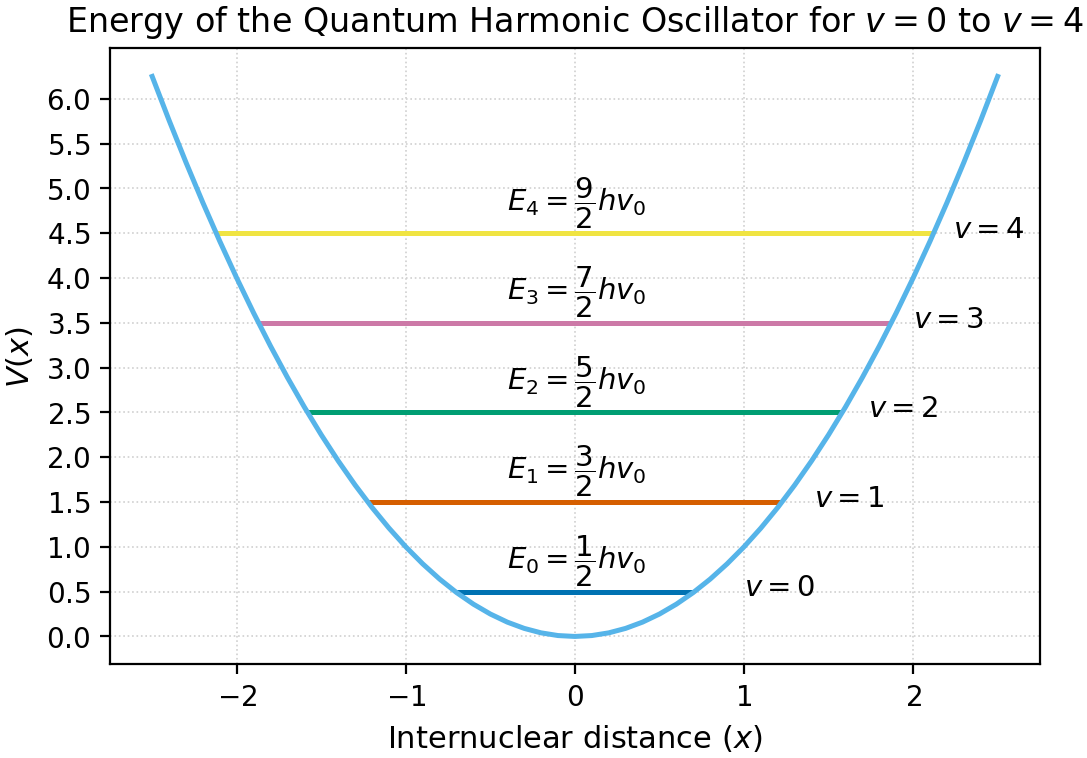
\includegraphics[width=0.5\linewidth]{Energy_levels}
  \caption{Skjematisk figur for temaet.}
  \label{fig:sirkel}
\end{figure}

Ved jevn sirkelbevegelse har sentripetalakselerasjonen
størrelsen $a_s = v^2/r$, rettet inn mot sentrum av sirkelen.


% =================================================
% OPPGAVE
% =================================================
\begin{exercise}
En satellitt går i en sirkulær bane med radius $r$ rundt en
planet med masse $M$.

\begin{enumerate}
  \item Vis at banehastigheten er $v = \sqrt{GM/r}$, hvor
        $G$ er Newtons gravitasjonskonstant.
  \item Uttrykk omløpstiden $T$ ved $r$, $M$ og $G$.
\end{enumerate}
\end{exercise}


\end{document}
